\documentclass[a4paper, 12pt]{book} % changed from scrbook
% not using \documentclass[a4paper, twoside=semi]{scrreprt} anymore

\usepackage{InfoSec}

\definecolor{bg}{RGB}{20,20,20}
\definecolor{fg}{RGB}{220,220,220}
\definecolor{keyword}{RGB}{130,170,255}
\definecolor{comment}{RGB}{120,120,120}
\definecolor{string}{RGB}{255,200,120}

\lstdefinestyle{darkbash}{
    backgroundcolor=\color{bg},
    basicstyle=\scriptsize\ttfamily\color{fg},
    keywordstyle=\color{keyword},
    commentstyle=\color{comment},
    autogobble=true,
    stringstyle=\color{string},
    breaklines=true,
    showstringspaces=false,
    frame=single
}

% \usepackage{titlesec}
% \setkomafont{chapter}{\Huge\bfseries}
% \setkomafont{section}{\Large\bfseries}
% \setkomafont{subsection}{\large\bfseries}
\usepackage{fancyhdr, lastpage}
\usepackage{lstautogobble}
\usepackage{euscript}


\makeatletter
\providecommand{\subtitle}[1]{\gdef\@subtitle{#1}}
\providecommand{\@subtitle}{}
\makeatother


\usepackage{booktabs}
\usepackage{array}
\usepackage{multirow}




\usepackage{newfloat}
%\usepackage{tocloft}

% % Define new float environment
% \DeclareFloatingEnvironment[
%   fileext=lof,
%   listname={List of Flowcharts},
%   name=Flowchart,
% ]{flowchart}


\pagestyle{fancy}
%\fancyhf{}
\lhead{}
\chead{}
%\rhead{Introduction to the Theory of Computation}
\cfoot{\thepage\ of \pageref{LastPage}}
\rfoot{Version 8.3}




\RequirePackage{etex} 


%--- The documentation for the title can be found at: https://en.wikibooks.org/wiki/LaTeX/Title_Creation
\title{Information Security \\ Cryptosystems}
\author{Ahmed U. Ashraf}
\date{\today }
% \subtitle{Version~\version}

\begin{document}

% \include{glossary}


\maketitle
%--- we would like to hyperlink each item in contensts page
% \let\hypercontentsline=\contentsline
% \renewcommand{\contentsline}[4]{\hypertarget{toc.#4}{}\hypercontentsline{#1}{#2}{#3}{#4}}
%--- We print ToC: Table of Contents

\DeclareFontShape{U}{stmry}{b}{n}{<-> ssub * stmry/m/n}{}

\tableofcontents\label{toc}
%--- We print the list of figures, this might go at the end.




% \listoffigures
% %--- We print the list of tables, this might also go at the end.
% \listoftables
% %--- This is to add list of symbols as glossary
% % \printunsrtglossary[type=symbols,style=long,title={List of Symbols}]


% % List of Algorithms (- taken the idea from Discrete Algorithmic Mathematics by Stephen B.Maurer and ANthony Ralston.pdf)

% \listofalgorithms
% \addcontentsline{toc}{chapter}{List of Algorithms}

% \listofflowcharts
% %\addcontentsline{toc}{chapter}{List of Flowcharts}











\emph{Cryptography} is the practice and study of techniques for secure communication in the presence of adverse third parties. \emph{Encryption} refers to the process of changing ordinary text (plaintext) into unintelligible text (ciphertext). \emph{Decryption} is the reverse.

% references: 
% 1. Introduction to Cryptography with Maple by Jose Luis Gomez Pardo
% 2. Introduction to Cybersecurity by Robin Sharp
% 3. Understanding Cryptography by Christof Paar, Jan Pelzl and Tim Guneysu
% 4. Introduction to Cryptography by Hans Delfs and Helmut Knebl
% 5. Introduction to Computer Networks and Cybersecurity by Chwan-Hwa Wu and J.David Irwin
% 6. Handbook of Financial Cryptography and Security by Biurton Rosenberg
% 7. Guide to Internet Cryptography by Jorg Schwenk
% 8. Guide to Computer Network Security by Joseph Migga Kizza
% 9. Encrypt, Sign, Attack by Olaf Manz
% 10. Cryptograpy Theory and Practice by Douglas R.Stinson
% 11. Discovering Cybersecurity by Seth James Nielson
% 12. CryptoSchool by Joachim von zur Gathen copy
% 13. Cryptology by Richard Klima and Neil Sigmon
% 14. Cryptography by Douglas R.Stinson and Maura B.Paterson
% 15. Cryptography and Network Security by William Stallings 
% 16. Cryptographic Protocol by Ling Dong and Kefei Chen
% 17. Cryptography and Network Security by Marcelo Sampaio de Alencar
% 18. Computer Security Fundamentals by Chuck Easttom
% 19. Computer Security and the Internet by Paul C.van Oorschot
% 20. Computer Security and Cryptography by Alan G.Konheim.pdf
% 21. CompTIA Security Certification Study Guide by Ahmed F.Sheikh
% 22. Classical and Modern Cryptography for Beginners by Rajkumar Banoth and Rekha Regar
% 23. A Classical Introduction to Cryptography by Serge Vaudenay



\chapter{Definition}

Let $\Sigma_1, \Sigma_2$ be alphabets \footnote{Plain and cipher alphabet.}, and let $\ell_1, \ell_2$ be positive integers. We are interested in functions of the form $f: \Sigma_1^{\ell_1} \longrightarrow \Sigma_2^{\ell_2}$

\begin{definition}
    A \emph{cryptosystem}\index{cryptosystem} or an \emph{encryption-decryption scheme}\index{encryption-decryption scheme} is a quintuple $\mathscr{C} = (\EuScript{P}, \EuScript{C}, \EuScript{K}, \EuScript{E}, \EuScript{D})$ where 
    \begin{enumerate}
        \item The collection $\EuScript{P} \subseteq \Sigma_1^{\ell_1}$ is the set of all possible \emph{plain texts}, called the \emph{plaintext space}. It consists of elementary strings that are to be encrypted as a basic unit.
        \item The collection $\EuScript{C}  \subseteq \Sigma_2^{\ell_2}$ is the set of all possible \emph{cipher texts}, called the \emph{ciphertext space}.
        \item The collection $\EuScript{K}$, called the \emph{key space}, is the set of all possible \emph{keys}. This may come along with a (\emph{keystream}) generator $g: \EuScript{K} \longrightarrow \Sigma^\infty$, where $\Sigma$ is the keystream alphabet.
        \item The collection $\EuScript{E} = (e_k: \EuScript{P} \rightarrow \EuScript{C})_{k \in \EuScript{K}}$\footnote{In case of haveing a keystream generator, the indexing set of encryption-decryption maps is the keystream space. So we sometime have abuse of notation where $\EuScript{K}$ means $\Sigma^{\infty}$.} is a finite set of \emph{encryption rules} $e_k$, that are functions given by polynomial-time algorithms.
        \item The collection $\EuScript{D} = (d_{k'}: \EuScript{C} \rightarrow \EuScript{P} )_{k' \in \EuScript{K}}$ is a finite set of \emph{decryption rules}, that are functions given by polynomial-time algorithms.
    \end{enumerate}
    such that for each \emph{encryption key} $k \in \EuScript{K}$, there exists a \emph{decryption key} $k' \in \EuScript{K}$, which satisfies
    \begin{align}
        d_{k'} \circ e_k \equiv 1_{\EuScript{P}}
    \end{align}
    That is, 
    \begin{align}
        d_{k'}(e_k(x)) = x
    \end{align}
    for all $x \in \EuScript{P}$.
\end{definition}


The plaintext and ciphertext messages are elements of $\EuScript{P}^*$ and $\EuScript{C}^*$, respectively. Given a plaintext message 
\begin{align}
    \mathbf{x} = x_1 x_2 \cdots x_{j}  \in \EuScript{P}^* \footnotemark 
\end{align}
and a cryptosystem $\mathscr{C}$, with encryption maps $e_k$, one can encrypt $\mathbf{x}$ with a key $k$ (as in \emph{Block cipher}\index{Block cipher}) by \footnotetext{These $x_i$ are in $\EuScript{P}$.}
\begin{align}
    \mathbf{y} = e_k(x_1) e_k(x_2) \cdots e_k(x_{j})
\end{align}
or with a key stream $k_1k_2\cdots $ (as in \emph{Stream cipher}\index{Stream cipher})  by
\begin{align}
    \mathbf{y} = e_{k_1}(x_1) e_{k_2}(x_2) \cdots e_{k_j}(x_j)
\end{align}

If the encryption key $k$ always equal to the decryption key $k'$ or if $k'$ is easily computed from $k$, then the cryptosystem is called \emph{symmetric}. If the encyrption and decryption keys $k, k'$ are not equal and computation of $k'$ is infeasible from $k$, then the cryptosystem is called \emph{assymetric}.







\section{Shift cipher}
\begin{definition}
    Let $G$ be an additive group (for example, $\mathbb{Z}$ or $\mathbb{Z}_n$). Let $\EuScript{P} = \EuScript{C} = G$ and $\EuScript{K}$ be a subset of $G$. Recall that $G$ acts on itself via translation (shift) and so does any subset, in particular $\EuScript{K}$, acts on $G$. We can define a \emph{shift cipher}, by setting:
    \begin{align}
        e_k(x) &\setn x + k 
    \end{align}
    and
    \begin{align}
        d_k(y) &\setn y - k 
    \end{align}
    That is $\bigg(G, G, G, (g \cdot)_{g \in G}, (g^{-1} \cdot)_{g \in G} \bigg)$\footnote{Here the group $G$ is written multiplicatively.} is called a \emph{shift cipher}.
\end{definition}


\begin{example}
    The usual English-alphabet shift cipher: Let $\EuScript{P} = \EuScript{C} = \EuScript{K} = \mathbb{Z}_{26}$. For $0 \leq k \leq 25$, define 
    \begin{align}
        e_k(x) &\setn x + k \pmod{26}
    \end{align}
    and 
    \begin{align}
        d_k(y) &\setn y - k \pmod{26} 
    \end{align}
    Consider the usual encoding $\{0,1,\ldots,25\} \equiv \{A, B, \ldots, Z\}$ and take $k = 3$, then this corresponds to the \textsf{Caeser} cipher \index{Caeser cipher}.
\end{example}

\begin{example}
    Consider the shift cipher for $k = 11$ on the plaintext message:
    \begin{align}
        \texttt{wewillmeetatmidnight}
    \end{align}
    We first use encoding to write it as
    \begin{align}
        \begin{array}{cccccccccc}
            22 & 4 & 22 & 8 & 11 & 11 & 12 & 4 & 4 & 19 \\
            0 & 19 & 12 & 8 & 3 & 13 & 8 & 6 & 7 & 19
        \end{array}
    \end{align}
    We apply the encryption
    \begin{align}
        \begin{array}{cccccccccc}
            7 & 15 & 7 & 19 & 22 & 22 & 23 & 15 & 15 & 4 \\
            11 & 4 & 23 & 19 & 14 & 24 & 19 & 17 & 18 & 4
        \end{array}
    \end{align}
    Converting back, we obtain
    \begin{align}
        \texttt{HPHTWWXPPELEXTOYTRSE}
    \end{align}

\end{example}





\section{Substitution cipher}

\begin{definition}
    If $\EuScript{P} = \EuScript{C}$ is a set, say $X$ and $\EuScript{K}$ $= \mathfrak{S}(X)$ that acts on $S$ via permutation, then we can define a \emph{substitution cipher}, by defining:
    \begin{align}
        e_\pi(x) &= \pi(x) 
    \end{align}
    and
    \begin{align}
        d_\pi(y) &= \pi^{-1}(x) 
    \end{align}
    That is $(X, X, \mathfrak{S}(X), g \cdot, g^{-1} \cdot)$\footnote{Here the group $G$ is written multiplicatively.} is called a \emph{shift cipher}.

\end{definition}






\begin{example}
    (\emph{English-alphabet}) \emph{Substitution Cipher}: Let $\EuScript{P} = \EuScript{C} = \mathbb{Z}_{26}$. Let $\EuScript{K}$ $= \mathfrak{S}_{26}$ consists of all possible permutations of $\{0,1,2,\ldots, 25\}$. For each permutation $\pi \in \EuScript{K}$, define
    \begin{align}
        e_\pi(x) = \pi(x)
    \end{align}
    and 
    \begin{align}
        d_\pi(y) &= \pi^{-1}(y)
    \end{align}
    where $\pi^{-1}$ is the inverse permutation to $\pi$. \textsf{Atbash cipher} is an example of a substitution cipher. 
\end{example}






\section{Affine cipher}

\begin{example}
    (\emph{English-alphabet}) \emph{Affine Cipher}: Let $\EuScript{P} = \EuScript{C} = \mathbb{Z}_{26}$, and let 
    \begin{align}
        \EuScript{K} &= \{(a, b) \in \mathbb{Z}_{26} \times \mathbb{Z}_{26}: \gcd(a, 26) = 1\}
    \end{align}
    For $k = (a, b) \in \EuScript{K}$, define 
    \begin{align}
        e_k(x) &= (ax + b) \pmod{26} 
    \end{align}
    and 
    \begin{align}
        d_k(y) &= a^{-1}(y - b) \pmod{26}
    \end{align}
    \textsf{ROT13} is an instance of an affine cipher.
\end{example}


\section{Hill cipher}
\begin{example}
        (\emph{English-alphabet}) \emph{Hill Cipher}: Let $m \geq 2$ be an integer and let $\EuScript{P} = \EuScript{C} = (\mathbb{Z}_{26})^m$, and let 
    % \begin{align}
    %     \EuScript{K} &= \mathrm{GL}_m(\mathbb{Z}_{26}) = \{m\times m~\text{invertible matrices over}~\mathbb{Z}_{26}\}
    % \end{align}
    For a key $A_k \in \EuScript{K}$, we define 
    \begin{align}
        e_k(x) &= A_k x
    \end{align}
    and 
    \begin{align}
        d_k(y) &= y A_k^{-1}
    \end{align}
    where all operations are performed over $\mathbb{Z}_{26}$.
\end{example}





\section{Permutation cipher}


A permutation cipher is a special case of a Hill cipher.
\begin{definition}
    Let $S$ be a set and let $\ell$ be a positive integer. Let $\EuScript{P} = \EuScript{C} = S^\ell$, and let $\EuScript{K}$ $= \mathfrak{S}_\ell$. For a key $\pi \in \mathfrak{S}_\ell$, we set
    \begin{align}
        e_{\pi}(x_1, x_2, \ldots, x_m) &\setn (x_{\pi_1}, x_{\pi_2}, \ldots, x_{\pi_m})
    \end{align}
    and
    \begin{align}
        d_{\pi}(y_1, y_2, \ldots, y_m) &\setn (y_{\pi^{-1}_1}, y_{\pi^{-1}_2}, \ldots, y_{\pi^{-1}_m})   
    \end{align}
\end{definition}




\section{Autokey cipher}


\section{Modes of Encryption}


\begin{enumerate}
    \item \emph{Electronic CodeBook}(ECB): is the simplest block cipher mode of operation. It divides plaintext into fixed -size blocks and encrypts each independently using the same key. Because identical plaintext blocks always produce identical ciphertext blocks, it fails to hide data patters and is generally insecure.
    \item \emph{Cipher Block Chaining}(CBC): xors the plaintext woth the prior ciphertext block. The first block must use an \emph{initialization vector}(IV) because there is no prior block.
    \item \emph{Cipher FeedBack mode} (CFB): 
    \item  \emph{Output FeedBack mode} (OFB).


\end{enumerate}





The following modes create a stream cipher from a block cipher. 
\begin{enumerate}
    \item CounTeR mode (CTR).
\end{enumerate}








\section{Terminology}
\emph{Cryptography} is the study of how to alter a message so that someone intercepting it cannot read it without the appropriate algorithm and key. Here are some terms associated with this that we would like to define before starting:
\begin{longtable}{|l|p{10cm}|} \hline 
    Cipher & A synonym for the algorithm used to transform plain text to cipher text. \\  \hline 
    Cipher text & The coded or encrypted message. If your encryption is sufficiently strong, your cipher text should be secure  \\ \hline 
    Cryptanalysis\footnote{Sometimes referred as \emph{code breaking}.} & the study of principles and methods of deciphering cipher text without knowing the key \\ \hline 
    Decipher (decrypt) & Decipher and decrypt are synonyms. Both terms mean to convert the cipher text to plain text. \\ \hline 
    Encipher (encrypt) &  Encipher and encrypt are synonyms. Both words mean to convert the plain text into cipher text. \\ \hline 
    Key & The information, usually some sort of number, used with the algorithm to encrypt or decrypt the message.  \\ \hline 
    Key space  & The total number of possible keys that could be used. \\ \hline 
    Plain text & The original message—the information you want to secure. \\ \hline 
\end{longtable}




















\section{Finite Field Arithmetic}


\section{Diffie-Hellman (DH) protocol}

Diffie-Hellman (DH) is a mathematical protocol\footnote{A protocol can also be thought as a special case of an algorithm.} that allows two parties to securely establish a shared secret over an insecure public network. Once generated, this shared secret is typically used as an encryption key for faster symmetric algorithms like AES to communicate privately.

DH is still in use today, but certain precautions have to be taken with respect to its building blocks. Authentication also needs to be implemented on top of DH to prevent man-in-the-middle threats.

The mathematical basis for this algorithm is Discrete Logarithm Problem (DLP).


\section{Rivest-Shamir-Adleman (RSA) protocol}

Rivest-Shamir-Adleman (RSA) is an asymmetric cryptographic algorithm used by modern computers that relies on factoring integers.



\section{Models of encryption}

\subsection{Symmetric encryption model}
\begin{figure}[H]
    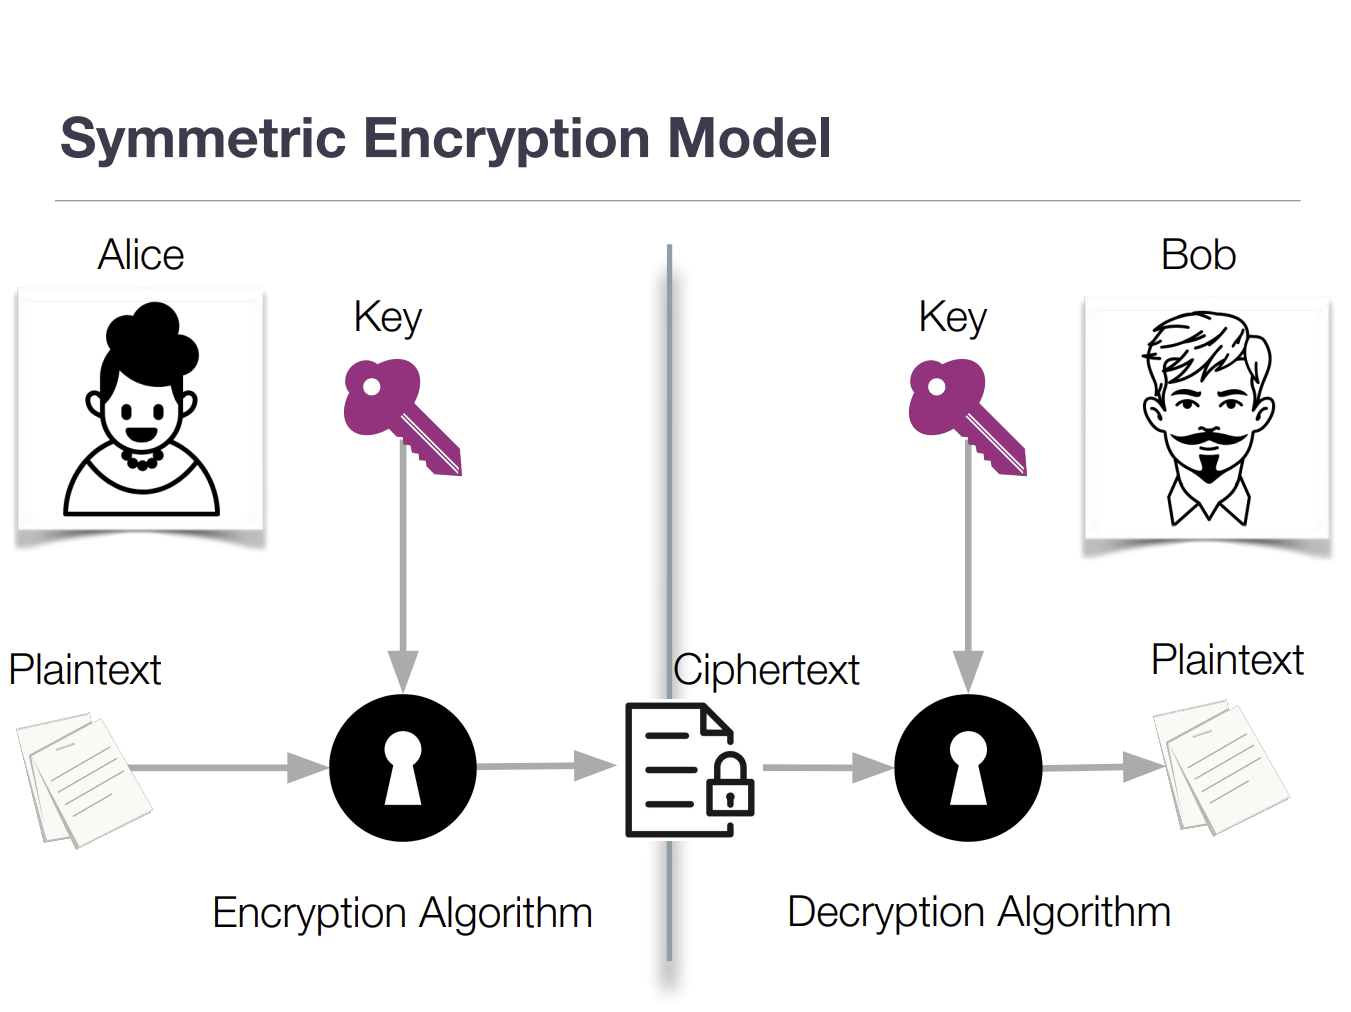
\includegraphics[scale=0.3]{symmetricmodel.png}
\end{figure}
The use cases for that are
\begin{enumerate}
    \item Web browsing using HTTPS.
    \item Encrypted chat (WhatsApp and Signal).
    \item Encrypted email (S/MIME and PGP).
    \item File and disk encryption.
\end{enumerate}

Requirements for symmetric encryption:
\begin{enumerate}
    \item Strong encryption.
    \item Fast.
    \item Sender and receiver must securely obtain and store secret key.
\end{enumerate}

\subsection{Public key encryption model}
\begin{figure}[H]
    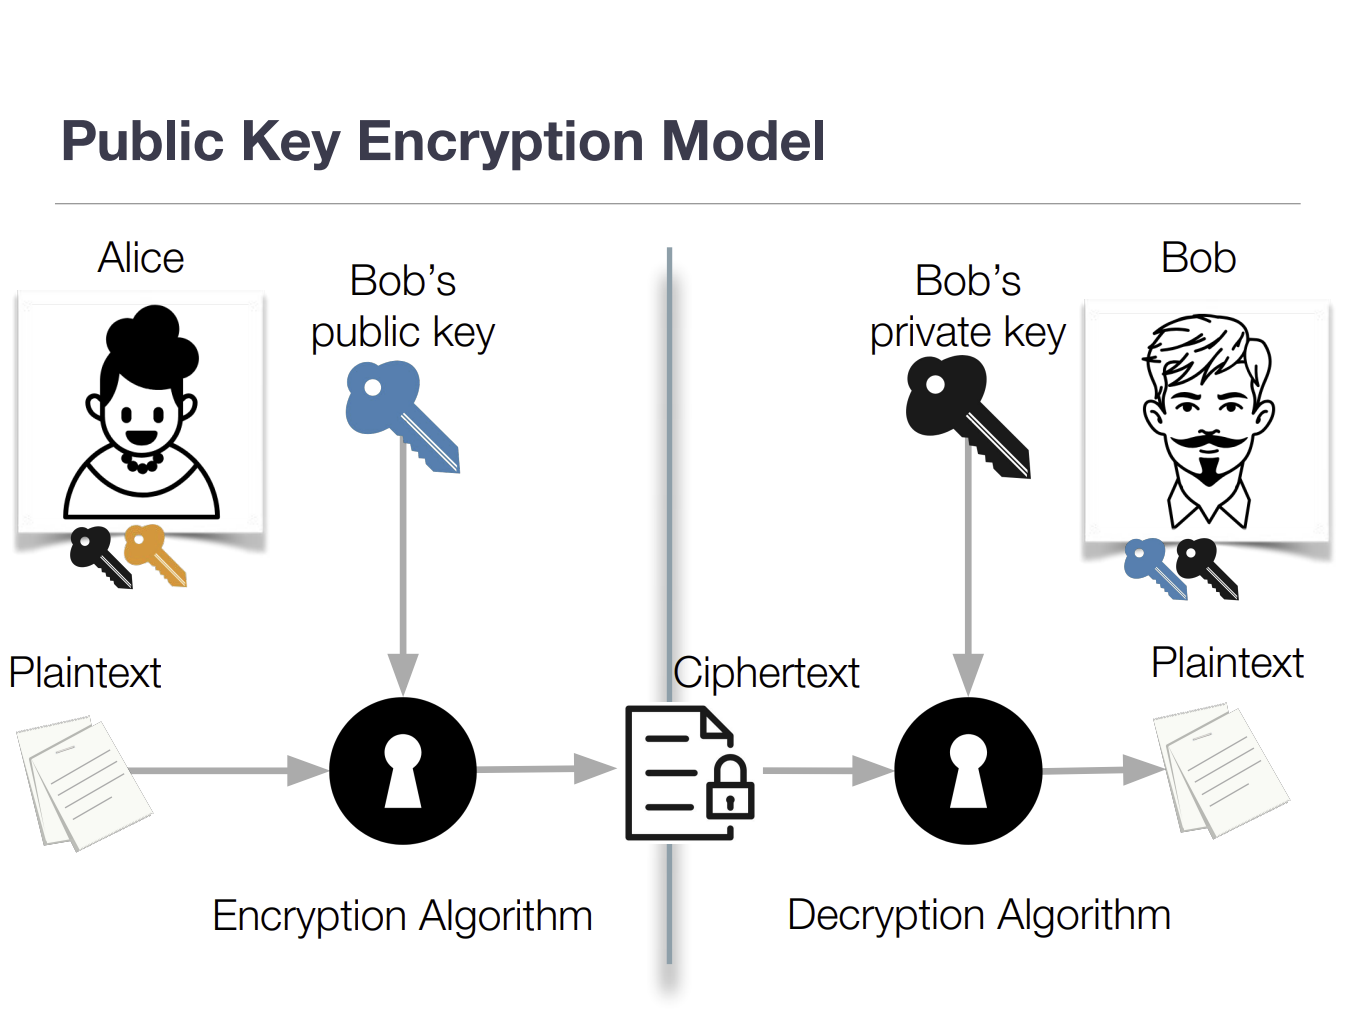
\includegraphics[scale=0.3]{publickey.png}
\end{figure}
The use cases for that
\begin{enumerate}
    \item Diffie-Hellman.
    \item RSA.
    \item Elliptic Curve Cryptography (ECC).
    \item Identity-based Encryption (IBE).
\end{enumerate}


\subsection{Public key digital signature model}
\begin{figure}[H]
    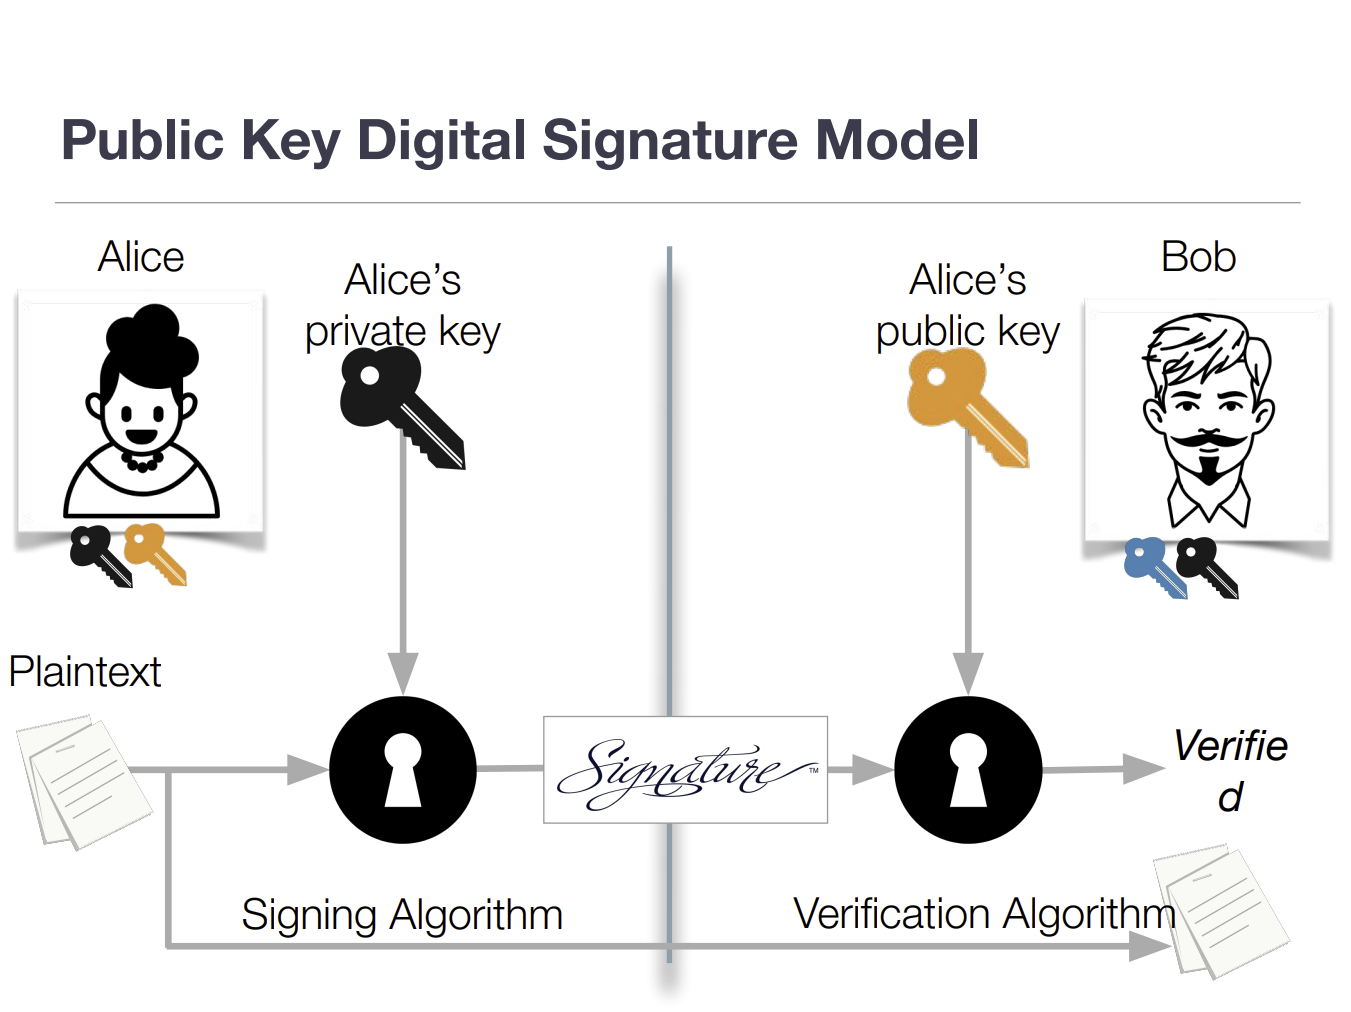
\includegraphics[scale=0.3]{publickeysign.png}
\end{figure}


\section{Cryptographic Hash Function}

These are one-way function\footnote{How can we make it rigorous.}. We desire the following properties from these functions, (call an arbitrary one $f$):
\begin{enumerate}
    \item It can be applied to a block of data of any size.
    \item It produces a fixed-length output.
    \item The value $f(x)$ is relatively easy to compute for any given $x$.
    \item \emph{One-way}: For any given value $h$, it is computationaly infeasible to find (any one of) its pre-image block $x$, that is such that $f(x) = h$.
    \item \emph{Weak collision resistant}: For any given block $x$, it is computationally infeasible to find $x' \neq x$ such that $f(x) = f(x')$.
    \item \emph{Strong collision resistant}: It is computationally infeasible to find any pair $(x, x')$ such that $f(x) = f(x')$.
\end{enumerate} 


Useful applications of hash function:
\begin{enumerate}
    \item Human-readable method to compare/verify data.
    \item Chaining events together - blockchain.
    \item Digital signatures and message authentication codes.
    \item Fundamental building block of many secure protocols.
\end{enumerate}

\begin{example}
    \emph{SHA-0}: Completely broken, collisions found.
    \emph{SHA-1}: Implemented using Merkle-Damg\.ard construction. 
    \emph{SHA-2}: No known flaws.
    \emph{SHA-3}: Subset of Keccak. Implemented using sponge construction.
\end{example}

\begin{example}
    \emph{MD5}: Completely broken, collisions found.
\end{example}














% \chapter{References}

%-- Computation Engineering by Ganesh Gopalakrishnan

\cite{adamson2012set}

% \nocite{*}



\bibliography{references}
\bibliographystyle{amsalpha}

\printindex




\end{document}